% !TeX spellcheck = id_ID
\documentclass[a4paper,12pt]{article}
\usepackage[bahasa]{babel}
\usepackage{graphicx}
\usepackage{multirow}
\usepackage{enumitem}
\usepackage{listings}
\usepackage{wrapfig}
\usepackage[T1]{fontenc}
\usepackage{inconsolata}
\usepackage{lipsum}
\usepackage{adjustbox}


\usepackage{color}
\usepackage[table]{xcolor}
\definecolor{pblue}{rgb}{0.13,0.13,1}
\definecolor{pgreen}{rgb}{0,0.5,0}
\definecolor{pred}{rgb}{0.9,0,0}
\definecolor{pgrey}{rgb}{0.46,0.45,0.48}
\lstset{language=Java,
	showspaces=false,
	showtabs=false,
	breaklines=true,
	showstringspaces=false,
	breakatwhitespace=true,
	commentstyle=\color{pgreen},
	keywordstyle=\color{pblue},
	stringstyle=\color{pred},
	rulecolor=\color{black},
	basicstyle=\ttfamily,
	moredelim=[il][\textcolor{pgrey}]{$$},
	moredelim=[is][\textcolor{pgrey}]{\%\%}{\%\%}
}

\graphicspath{ {./img/} }
\begin{document}
\title{ {\Large Laporan Praktikum}\\ Algoritma dan Pemrograman \\{\Large Pertemuan 9}}

\author{Aldzikri Dwijayanto Prathama 
	\\195410189
	\\Teknik Informatika}
\makeatletter
\begin{titlepage}
	\begin{center}
		{\huge \bfseries \@title }\\[14ex]
		
\includegraphics[scale=.8]{logo}\\[4ex]
		{\large \@author}\\[19ex]
		{\large \bfseries {SEKOLAH TINGGI MANAJEMEN INFORMATIKA DAN KOMPUTER
				AKAKOM YOGYAKARTA}}
	\end{center}


%{\large \@date} 
\end{titlepage}
\makeatother
%\maketitle
\newpage
\tableofcontents
\newpage

\section{Tujuan}
Mahasiswa dapat mengimplementasikan konsep perulangan do-while untuk menyelesaikan kasus

\section{Dasar Teori}
\paragraph{}
Perintah ini sangat mirip dengan perintah while, perbedaannya adalah bahwa pada perintah while pemeriksaan ekspresi logika dilakukan di awal, jadi jika ekspresi bernilai false maka pengulangan tidak akan dijalankan sama sekali, namun pada perintah do – while ini pemeriksaan dilakukan di akhir kalang (loop) sehingga walaupun sejak awal ekspresi akan bernilai false maka minimal kalang (loop) akan dieksekusi sekali. Seperti pada perintah while proses pengulangan akan berjalan jika kondisi yang diperiksa pada while masih bernilai benar dan pengulangan akan dihentikan jika kondisinya sudah bernilai salah.\\
Sintaks penulisannya sebagai berikut :
\begin{lstlisting}[frame=single]
do
{
  Pernyataan;

}while(ungkapan);

\end{lstlisting}

Keterangan :
\begin{itemize}[label={-}]
	\item Bagian pernyataan dijalankan secara berulang sampai ungkapan bernilai salah.
	
	\item Pengujian ungkapan dilakukan setelah bagian pernyataan, maka pada pernyataan do ... while minimal akan dijalankan sekali, karena begitu masuk ke blok perulangan, tidak ada cek kondisi tetapi langsung mengerjakan pernyataan.
\end{itemize}

\section{Praktik}

\subsection{Praktik 1}
\begin{enumerate}
	 

\item \begin{minipage}[t]{\linewidth}
	\raggedright
	\adjustbox{valign=t}{%
	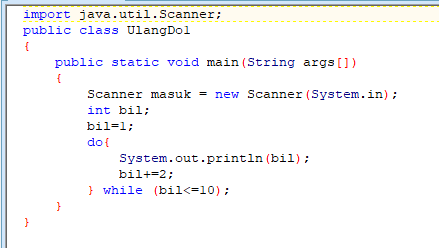
\includegraphics[scale=1]{Capture1}
	}
\begin{center}
	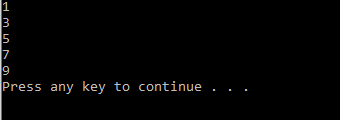
\includegraphics[scale=1]{Capture1_2}
\end{center}


    \end{minipage}
Pada program java di atas, variabel bil dideklarasikan sebagai integer dengan nilai 1, setelah itu terdapat pengulangan do-while, dengan pernyataan yang akan mengeluarkan nilai dari variabel bil ke layar, lalu akan menambah variabel bil dengan 2. Pengulangan akan terus dilakukan hingga variabel bil <= 10, seperti kondisi yang ada pada while.

\item \begin{minipage}[t]{\linewidth}
	\raggedright
	\adjustbox{valign=t}{%
		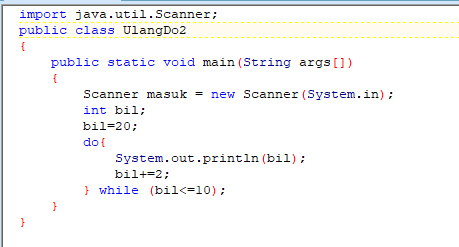
\includegraphics[scale=1]{Capture2}
	}
	\begin{center}
		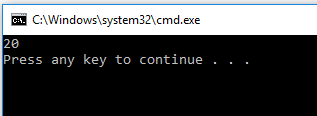
\includegraphics[scale=1]{Capture2_2}
	\end{center}
	
	
\end{minipage}
Pada program java di atas, variabel bil dirubah nilainya menjadi 20, hasilnya program  menge-print nilai variabel bil ke layar, lalu program akan berhenti, ini karena pengulangan do-while melakukan perulangan terlebih dahulu sebelum melakukan pemeriksaan kondisi. Maka outputnya program akan mengeluarkan angka 20 dari layar yang mana adalah nilai dari variabel bil, lalu akan berhenti.

\end{enumerate}

\subsection{Praktik 2}
\begin{center}
	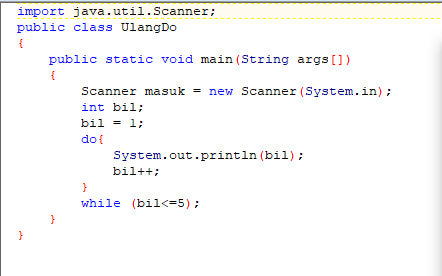
\includegraphics[scale=1]{Capture3}
	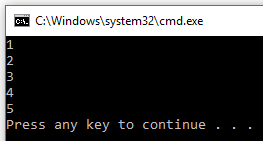
\includegraphics[scale=1]{Capture3_2}
\end{center}
Program java UlangDo dari praktik 2 memiliki variabel integer bil bernilai 1, lalu memiliki perulangan do-while. Perulangan tersebut memiliki pernyataan yang mana akan mengeluarkan nilai dari variabel nilai ke layar, lalu akan menambah nilai variabel bil dengan 1, disetiap perulangannya, setelah itu perulangan do-while akan memeriksa kondisi, adapun kondisi tersebut, adalah bil<=5. Jadi program akan berhenti jika variabel bil sudah memiliki nilai lebih besar dari 5. Output dari program menghasilkan hitung mundur dari 1 sampai 5.

\subsection{Praktik 3}
\begin{center}
	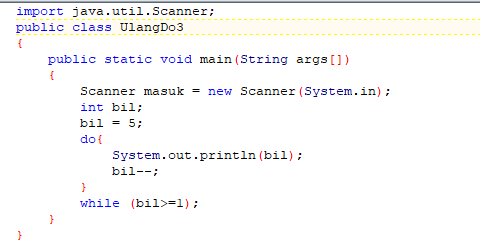
\includegraphics[scale=1]{Capture4}
	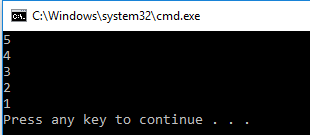
\includegraphics[scale=1]{Capture4_2}
\end{center}

Praktik 3 meminta mahasiswa untuk merubah program dari praktik 2 agar menghasilkan output hitung mundur, dari 5 sampai 1.
Agar program dari praktik 2 menghasilkan perhitungan mundur, yang perlu kita ganti adalah nilai bil menjadi berniali 5, lalu bil++ dirubah menjadi bil--, dan kondisi di while bil<=5 menjadi bil>=1.\\
jadi program akan melakukan menge-print niali dari variabel bil, lalu mengurangi nilainya dengan 1 di setip perulangan, dan perulangan akan terus berjalan selama variabel bil memiliki nilai >= 1.

\subsection{Praktik 4}
\begin{center}
	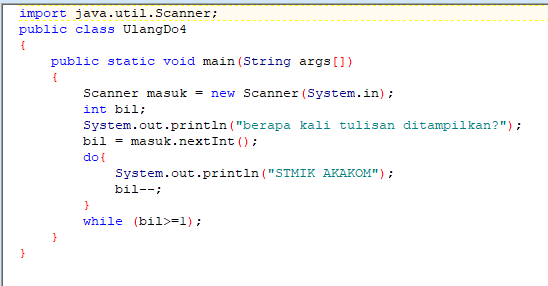
\includegraphics[scale=1]{Capture5}
	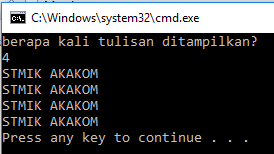
\includegraphics[scale=1]{Capture5_2}
\end{center}

Program java UlangDo4 memiliki variabel bil berjenis integer, yang nilainya dimasukkan oleh user, lalu terdapat perulangan do-while dengan pernyataan yang akan mengeluarkan tulisan "STMIK AKAKOM" ke layar, lalu akan mengurangi nilai dari variabel bil dengan 1, yang akan terus diulang selama variabel bil lebih besar dari sama dengan 1. Sehingga program akan mengeluarkan tulisan "STMIK AKAKOM" sebanyak angka yang  dimasukkan leh user ke layar.

\section{Latihan}
\subsection{Latihan 1}
\begin{center}
	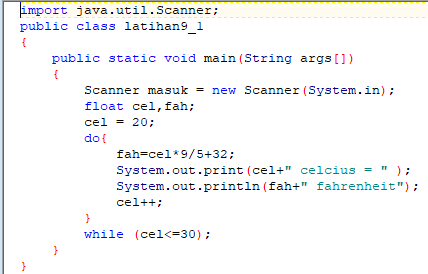
\includegraphics[scale=1]{Capture6}
	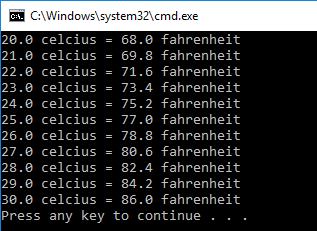
\includegraphics[scale=1]{Capture6_2}
\end{center}
Pada program latihan9\_1 di atas, terdapat variabel cel yang bernilai 20 dan fah yang berjenis float, lalu di bawahanya terdapat perulangan do-while yang akan menjalankan operasi konversi cel ke fahrenheit dan memasukan hasilnya ke variabel fah, lalu program akan menampilkan nilai dari variabel cel dan fah, setelah itu akan menambahkan nilai 1, ke variabel cel. Perulangan ini akan terus diulang selama variabel bernilai kurang dari sama dengan 30. Sehingga program tersebut akan menampilkan suhu celcius dari 20 - 30 dan mengkonversinya ke fahrenheit.

\subsection{Latihan 2}
\begin{center}
	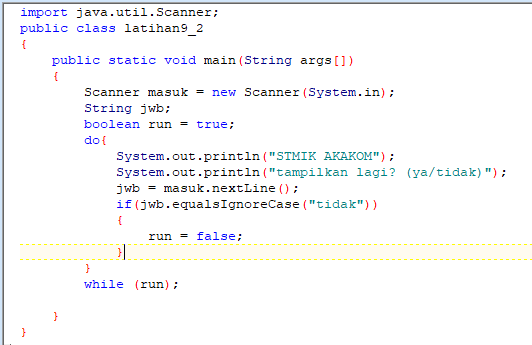
\includegraphics[scale=1]{Capture7}
	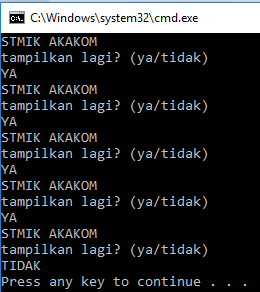
\includegraphics[scale=1]{Capture7_2}
\end{center}
Program latihan9\_2 memiliki variabel jwb yang berjenis string, dan run yang bernilai true dan berjenis boolean. Dibawahnya terdapat perulangan do-while yang akan menampilkan tulisan "STMIK AKAKOM"  ke layar, lalu akan menyediakan input untuk user, kika user memasukkan tidak, maka variabel dari run akan berubah menjadi false, sehingga kondisi di while tidak terpenuhi dan perulanganpun berhenti.

\section{Tugas}
\subsection{Tugas 1}
\begin{center}
	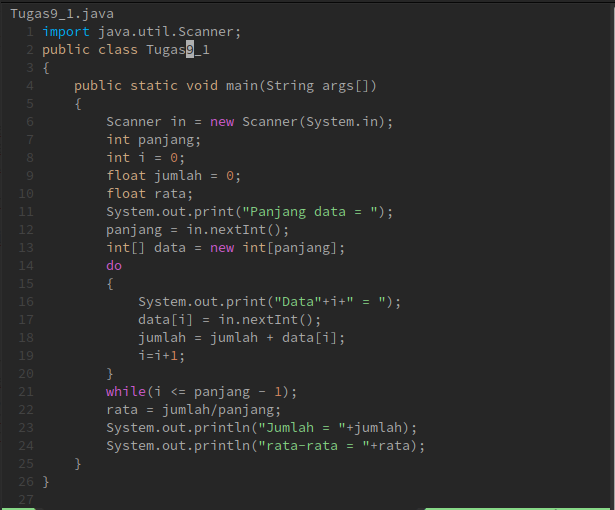
\includegraphics[scale=.5]{tugas1}
	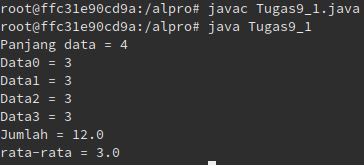
\includegraphics[scale=.5]{tugas1_2}
\end{center}
Program di atas memiliki variabel \texttt{data} yang berbentuk array integer, yang panjangnya ditentukan oleh variabel panjang. Karena array di java bersifat tetap, maka digunakan ArrayList, terlihat pada baris kode
\begin{lstlisting}
int[] data = new int[panjang];
\end{lstlisting}   
baris ini akan merubah panjang variabel \texttt{data}, dengan nilai dari variabel \texttt{panjang}.\\
Pada fungsi \texttt{while} diberi kondisi i <= panjang - 1, itu karena array dimulai dari 0, jadi misalnya kita memberi panjang array itu 4, maka akan terdiri dari 0, 1, 2, 3.\\
Di dalam \texttt{do} terdapat pernyataan
\begin{lstlisting}
data[i] = in.nextInt();
\end{lstlisting}
pernyataan ini akan menerima masukan dan memasukkannya ke variabel \texttt{data} ke "i", jadi variabel \texttt{data} akan dapat dimasukkan nilai sesuai dengan panjang array yang telah ditentukan.\\
Lalu baris pernyataan
\begin{lstlisting}
jumlah = jumlah + data[i];
\end{lstlisting}
berfungsi untuk menambahkan variabel \texttt{jumlah}, dengan nilai variabel \texttt{data} ke "i", jadi variabel \texttt{jumlah} akan bernilai jumlah semua angka yang ada di variabel \texttt{data}.\\
Setelah perulangan do-while selesai, program akan menjalankan pernyataan
\begin{lstlisting}
rata = jumlah/panjang;
\end{lstlisting}
yang akan memberi nilai ke variabel \texttt{rata} dari hasil operasi pembagian jumlah dengan panjang, yang menghasilkan rata-rata dari semua nilai di variabel \texttt{data}

\subsection{Tugas 2}
\begin{center}
	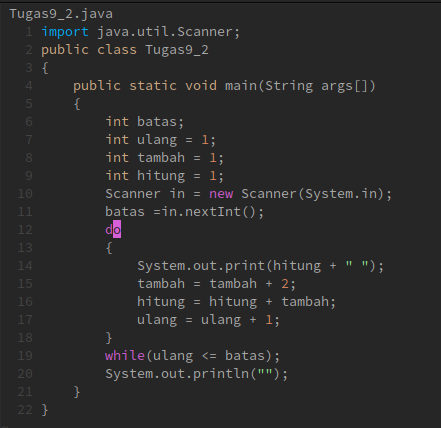
\includegraphics[scale=.5]{tugas2}
	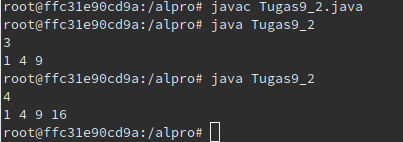
\includegraphics[scale=.5]{tugas2_2}
\end{center}
Pada program di atas terdapat pengulangan do-while yang memiliki kondisi ulang <= batas, yang mana variabel \texttt{ulang} dideklarasikan di awal memiliki nilai 1, dan variabel \texttt{batas} dimasukkan oleh user.
karena deret bilangan 1, 4, 9, 16 memiliki selisih 3, 5, 7, yang juga memiliki selisih masing-masing bilangan yaitu 2. Maka variabel \texttt{tambah} ditambah dengan bilangan 2 di setiap perulangan, lalu variabel hitung ditambahkan dengan variabel tambah di setiap perulangan, setelah itu variabel ulang ditambah dengan 1, agar perulangan berhenti sesuai dengan variabel \texttt{batas} yang nilainya dimasukkan user.

\newpage

\section{Kesimpulan}
Setelah kegiatan praktik mahasiswa dapat mengimplementasikan konsep perulangan do-while untuk menyelesaikan kasus

\end{document}